%% pba_to_campy_ecoli.tex
%% Author: Leighton Pritchard
%% Copyright: James Hutton Institute
%% These slides describe two endpoints to my career in bacterial genome
%% sequencing: Pectobacterium atrosepticum, and the recent Campylobacter
%% and E.coli sequencing work. 
%% The aim here is to contrast in broad terms the two different ends of the scale,
%% and illustrate how far we've moved on in terms of technology and scale
%% for sequencing, with a bit of personal background.

% SUBSECTION: A personal view
% How I went from a very large sequencing project for one bacterium, to 
% many sequencing projects for thousands of bacteria
\subsection{A personal view}

% The merest summary of the impact of sequencing
\begin{frame}
  \frametitle{The impact\footnote{\tiny{Loman and Pallen (2015) \textit{Nat. Rev. Micro.} \href{http://dx.doi.org/10.1038/nrmicro3565}{doi:10.1038/nrmicro3565}}}}
  Genome sequencing and bioinformatics have transformed our understanding of prokaryotic biology:
  \begin{itemize}
    \item function
    \item evolution
    \item interactions
    \item community structure
    \item real-time monitoring and diagnostics
    \item as a platform for synthetic biology
  \end{itemize}
  It now takes much longer to analyse than generate data
\end{frame}

% Outline the two extremes I'll talk about (briefly)
\begin{frame}
  \frametitle{The endpoints}
  \begin{itemize}
    \item \textbf{2003}: \textit{Erwinia carotovora} subsp. \textit{atroseptica}
    \item \textbf{2015}: \textit{Dickeya} spp., \textit{Campylobacter} spp., and \textit{Escherichia coli}
  \end{itemize}
      \begin{center}
        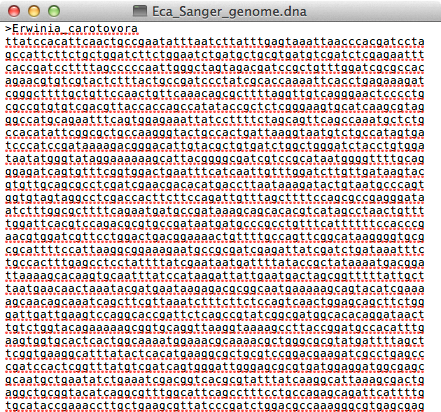
\includegraphics[height=0.5\textheight]{images/pba_sequence}
        
\includegraphics[width=0.5\textheight]{images/campy_presence_absence}
      \end{center}      
\end{frame}

% Pba
\subsection{Erwinia carotovora subsp. atroseptica}

% The sequencing project, and what we got out of it
\begin{frame}
  \frametitle{2003: \textit{E. carotovora} subsp. \textit{atroseptica}}
  \begin{itemize}
    \item \textbf{ \pounds250k collaboration} between SCRI, University of Cambridge, WT Sanger Institute
    \item Single isolate: \textit{E. carotovora} subsp. \textit{atroseptica} SCRI1043
    \item The first sequenced enterobacterial plant pathogen (32 authors!) \footnote{\tiny{Bell \textit{et al}. (2004) \textit{Proc. Natl. Acad. Sci. USA} \textbf{101}: \textbf{30}:11105-11110. \href{http://dx.doi.org/10.1073/pnas.0402424101}{doi:10.1073/pnas.0402424101}}}\\ 
      \begin{center}
        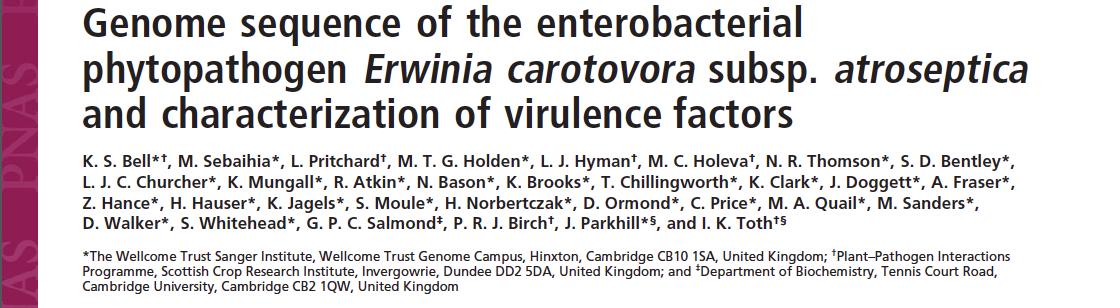
\includegraphics[width=0.6\textwidth]{images/pba_pnas}
      \end{center}    
    \item All repeats and gaps bridged and sequenced directly
    \item \textbf{Result}: a single, complete, high-quality 5Mbp circular chromosome at 10.2X coverage: 106,500 reads
  \end{itemize}
\end{frame}

% The effort that went into annotation
\begin{frame}
  \frametitle{2003: \textit{E. carotovora} subsp. \textit{atroseptica}}
  A genome sequence is a starting point$\ldots$
  \begin{itemize}
    \item Manual annotation by the Sanger Pathogen Sequencing Unit
    \item Literature searches and comparisons
    \item \textbf{Six people, for six months $\approx$ three person-years}
    \item Genes: \texttt{BLAST}, \texttt{GLIMMER}, \texttt{ORPHEUS}
    \item Functional domains: \texttt{PFAM}, \texttt{SIGNALP}, \texttt{TMHMM}
    \item Metabolism: \texttt{KEGG}
    \item ncRNA: \texttt{RFAM}
  \end{itemize}
\end{frame}

% Annotation files
\begin{frame}
  \frametitle{2003: \textit{E. carotovora} subsp. \textit{atroseptica}}
  Working (\url{Eca_Sanger_annotation.gbk}) and published (\url{NC_004547.gbk}) annotation files are in the \texttt{data} directory
  \begin{center}
    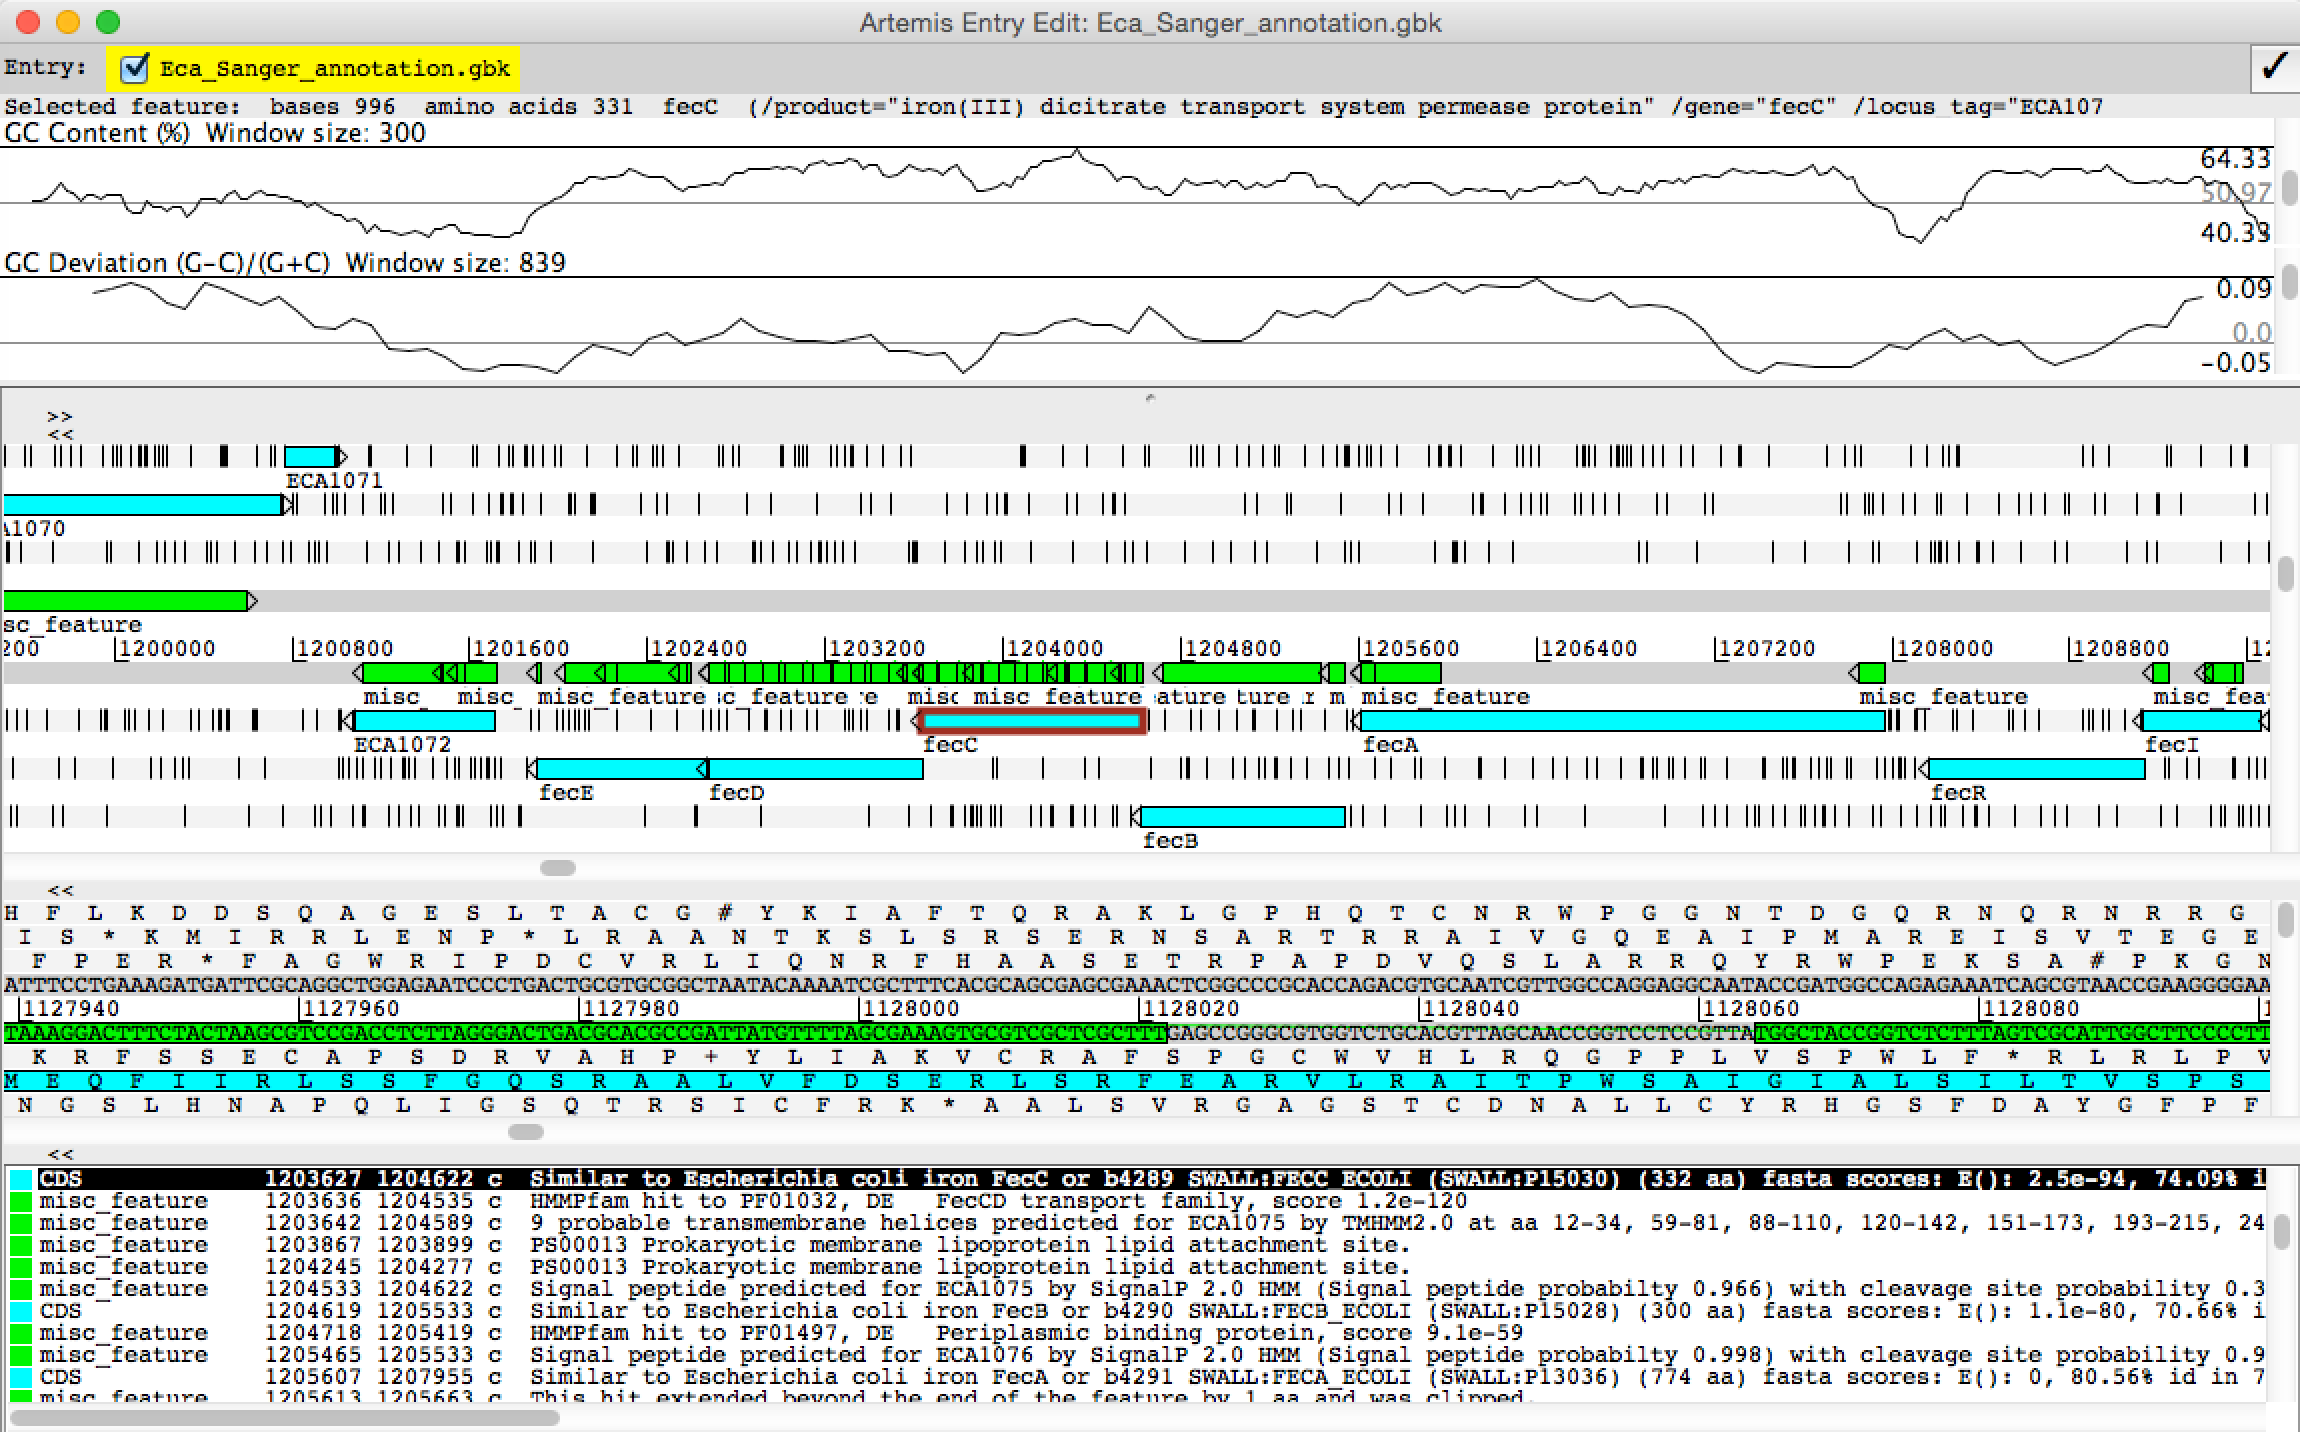
\includegraphics[width=0.9\textwidth]{images/pba_artemis}
  \end{center}    
\end{frame}

% The comparative genomics
\begin{frame}
  \frametitle{2003: \textit{E. carotovora} subsp. \textit{atroseptica}}
  Compared against all 142 available bacterial genomes\footnote{\tiny{\url{data/Pba} directory in the accompanying GitHub repository}}
  \begin{center}
    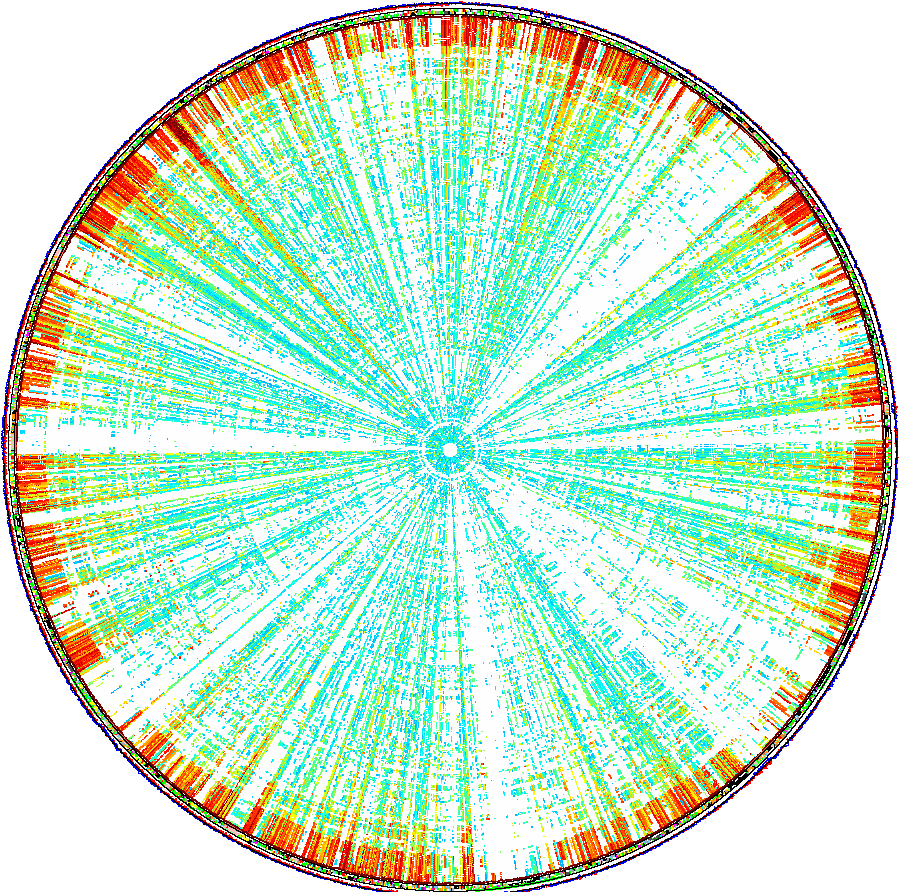
\includegraphics[width=0.6\textwidth]{images/pba_400_circular}
  \end{center}    
\end{frame}

% Dickeya etc
\subsection{Dickeya spp., Campylobacter spp., and Escherichia coli}

% Dickeya sequencing summary
\begin{frame}
  \frametitle{2013: \textit{Dickeya} spp.}
  Sequenced and annotated 25 new isolates of \textit{Dickeya}
  \begin{itemize}
    \item 25 \textit{Dickeya} isolates, at least six species
    \item Multiple sequencing methods: 454, Illumina (SE, PE)
    \item Minor publications (6, 8 authors)%
\footnote{\tiny{Pritchard \textit{et al}. (2013) \textit{Genome Ann.} \textbf{1} (4) \href{http://dx.doi.org/10.1128/genomeA.00087-12}{doi:10.1128/genomeA.00087-12}}}$^{,}$%
\footnote{\tiny{Pritchard \textit{et al}. (2013) \textit{Genome Ann.} \textbf{1} (6) \href{http://dx.doi.org/10.1128/genomeA.00978-13}{doi:10.1128/genomeA.00978-13}}}\\ 
      \begin{center}
        
\includegraphics[width=0.5\textwidth]{images/dickeya_ga1}
        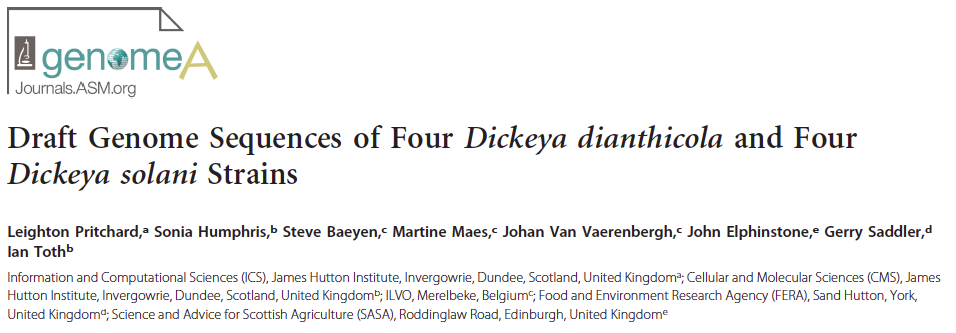
\includegraphics[width=0.5\textwidth]{images/dickeya_ga2}
      \end{center}    
    \item \textbf{Results}: 12-237  fragments containing 4.2-5.1Mbp, at 6-84X coverage, 170k-4m reads
    \item \textbf{Automated annotation: RAST} with manual corrections
  \end{itemize}  
\end{frame}

% Dickeya sequencing summary
\begin{frame}
  \frametitle{2013: \textit{Dickeya} spp.}
  Within-genus comparisons: large-scale synteny and rearrangement
  \begin{center}
    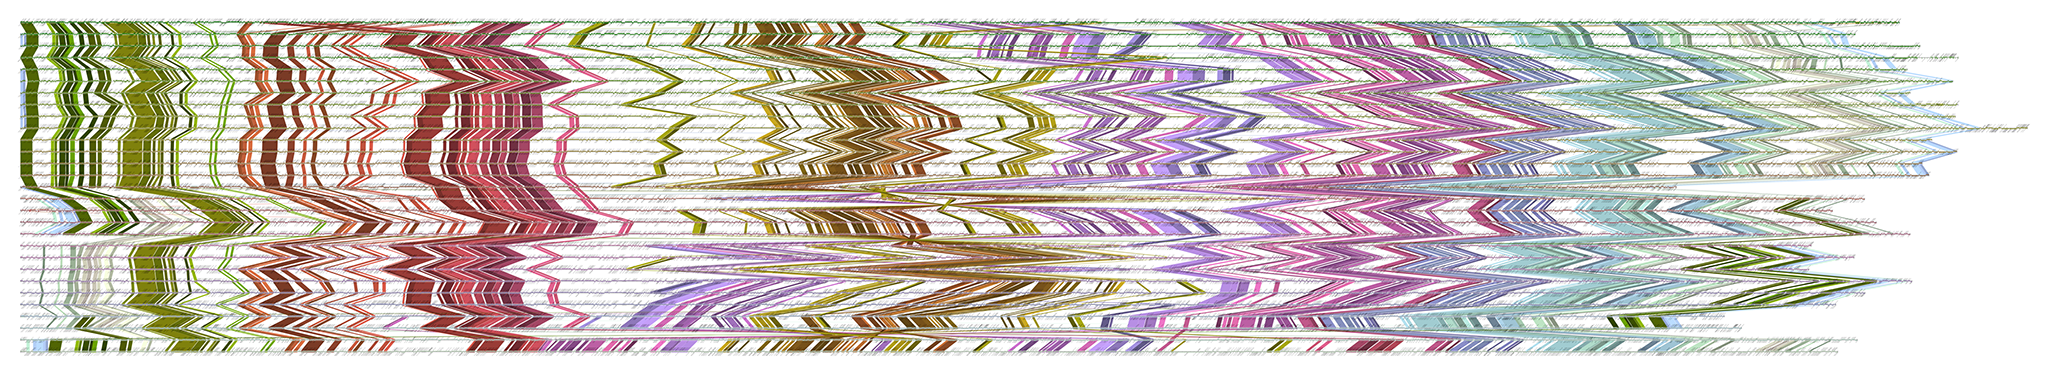
\includegraphics[width=1\textwidth]{images/dickeya_core_collinear_small}
  \end{center}    
  Within-species comparisons: e.g. indels, HGT
  \begin{center}
    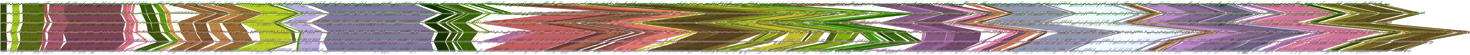
\includegraphics[width=1\textwidth]{images/collinear_zeae}
  \end{center}      
\end{frame}

% Dickeya sequencing summary
\begin{frame}
  \frametitle{2013: \textit{Dickeya} spp.}
  Within-genus comparisons: whole genome-based species delineation\footnote{\tiny{\href{http://dx.doi.org/10.1099/ijs.0.052944-0}{van der Wolf \textit{et al}. (2014) \textit{Int. J. Syst. Evol. Micr.} \textbf{64}:768-774 doi:10.1099/ijs.0.052944-0}}}
  \begin{center}
    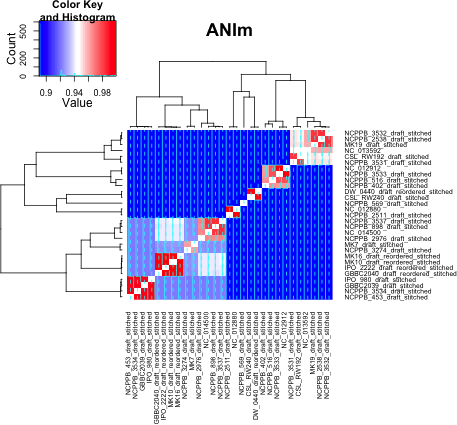
\includegraphics[width=0.6\textwidth]{images/dickeya_ani}
  \end{center}      
\end{frame}

% Dickeya sequencing summary
\begin{frame}
  \frametitle{2013: \textit{Dickeya} spp.}
  Within-genus comparisons: differences in metabolism
  \begin{center}
    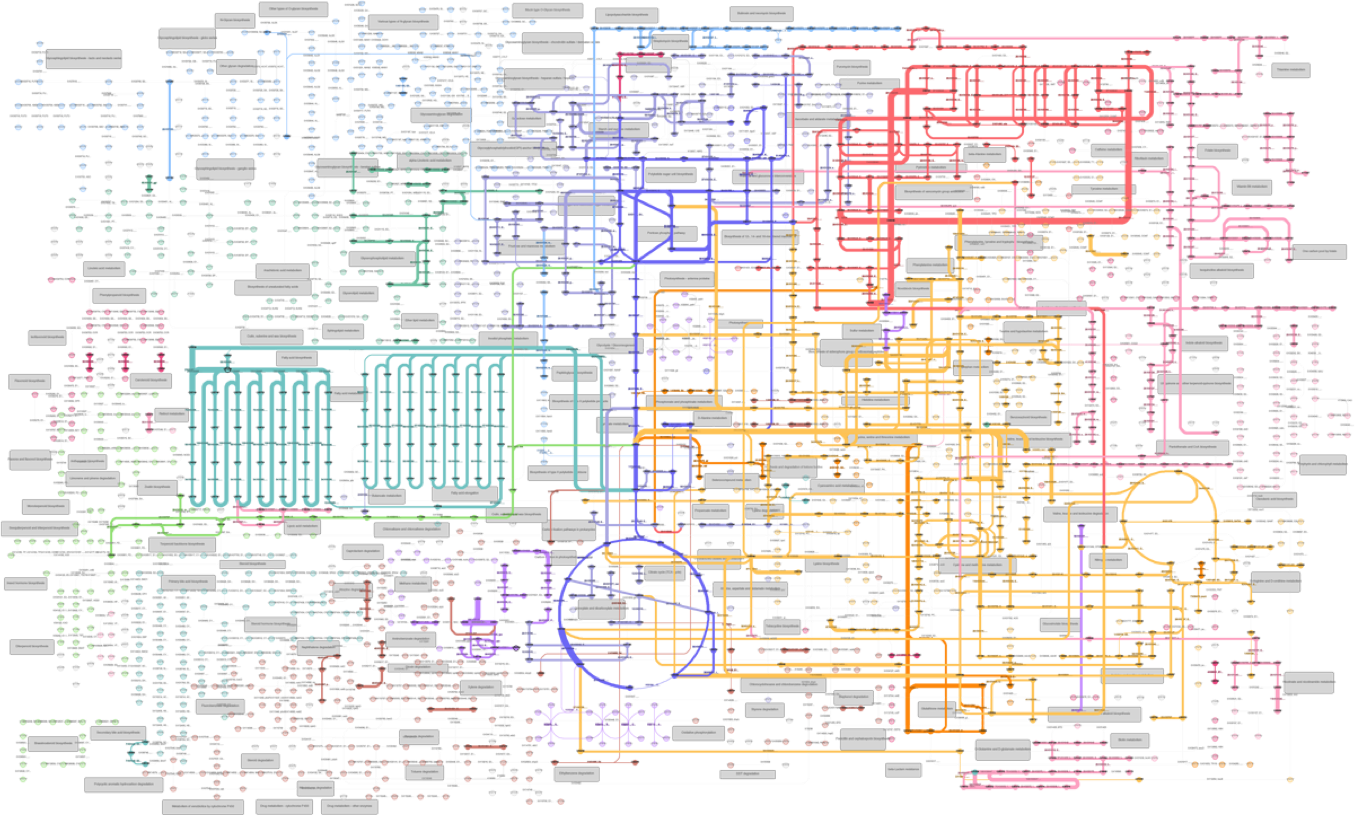
\includegraphics[width=1\textwidth]{images/dickeya_metabolism}
  \end{center}      
\end{frame}

% E.coli sequencing summary
\begin{frame}
  \frametitle{2014: \textit{E. coli}}
  Sequenced and annotated $\approx$ 190 isolates of \textit{E. coli} \\
  All bacteria environmental, sampled from lysimeters
  \begin{itemize}
    \item Illumina paired-end sequencing. \textbf{Total cost of sequencing 190 bacteria: $\approx$\pounds11k}
    \item \textbf{Automated annotation: PROKKA}
  \end{itemize}  
\end{frame}

% E.coli sequencing variation
\begin{frame}
  \frametitle{2014: \textit{E. coli}}
  Sequencing output variable - even though same preps, ``same'' bacteria, similar sources.
  \begin{itemize}
    \item \textbf{Results}: 5-3000 contigs (median $\approx$ 125); 9kbp-7.1Mbp (median $\approx$ 5Mbp); 170k-4m reads
  \end{itemize}  
  \begin{center}
    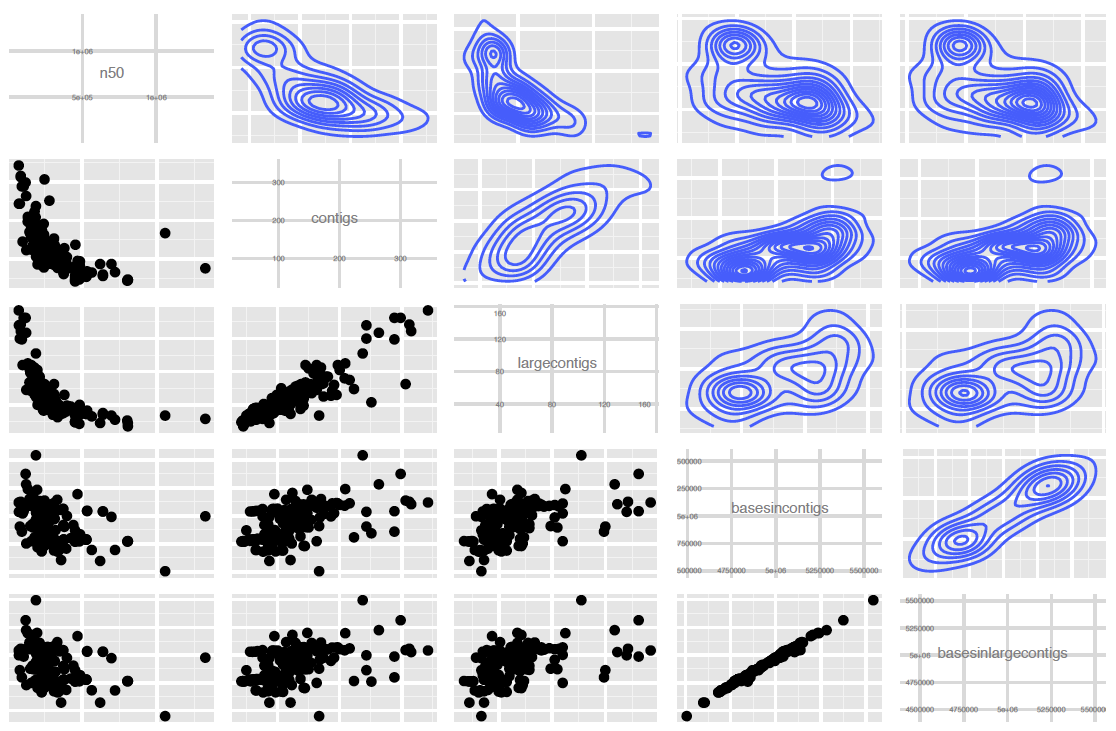
\includegraphics[width=0.7\textwidth]{images/ecoli_sequencing_variation}
  \end{center}      
\end{frame}

% E.coli within-species variation
\begin{frame}
  \frametitle{2014: \textit{E. coli}}
  Genome sequencing enables within-species classification
  \begin{center}
    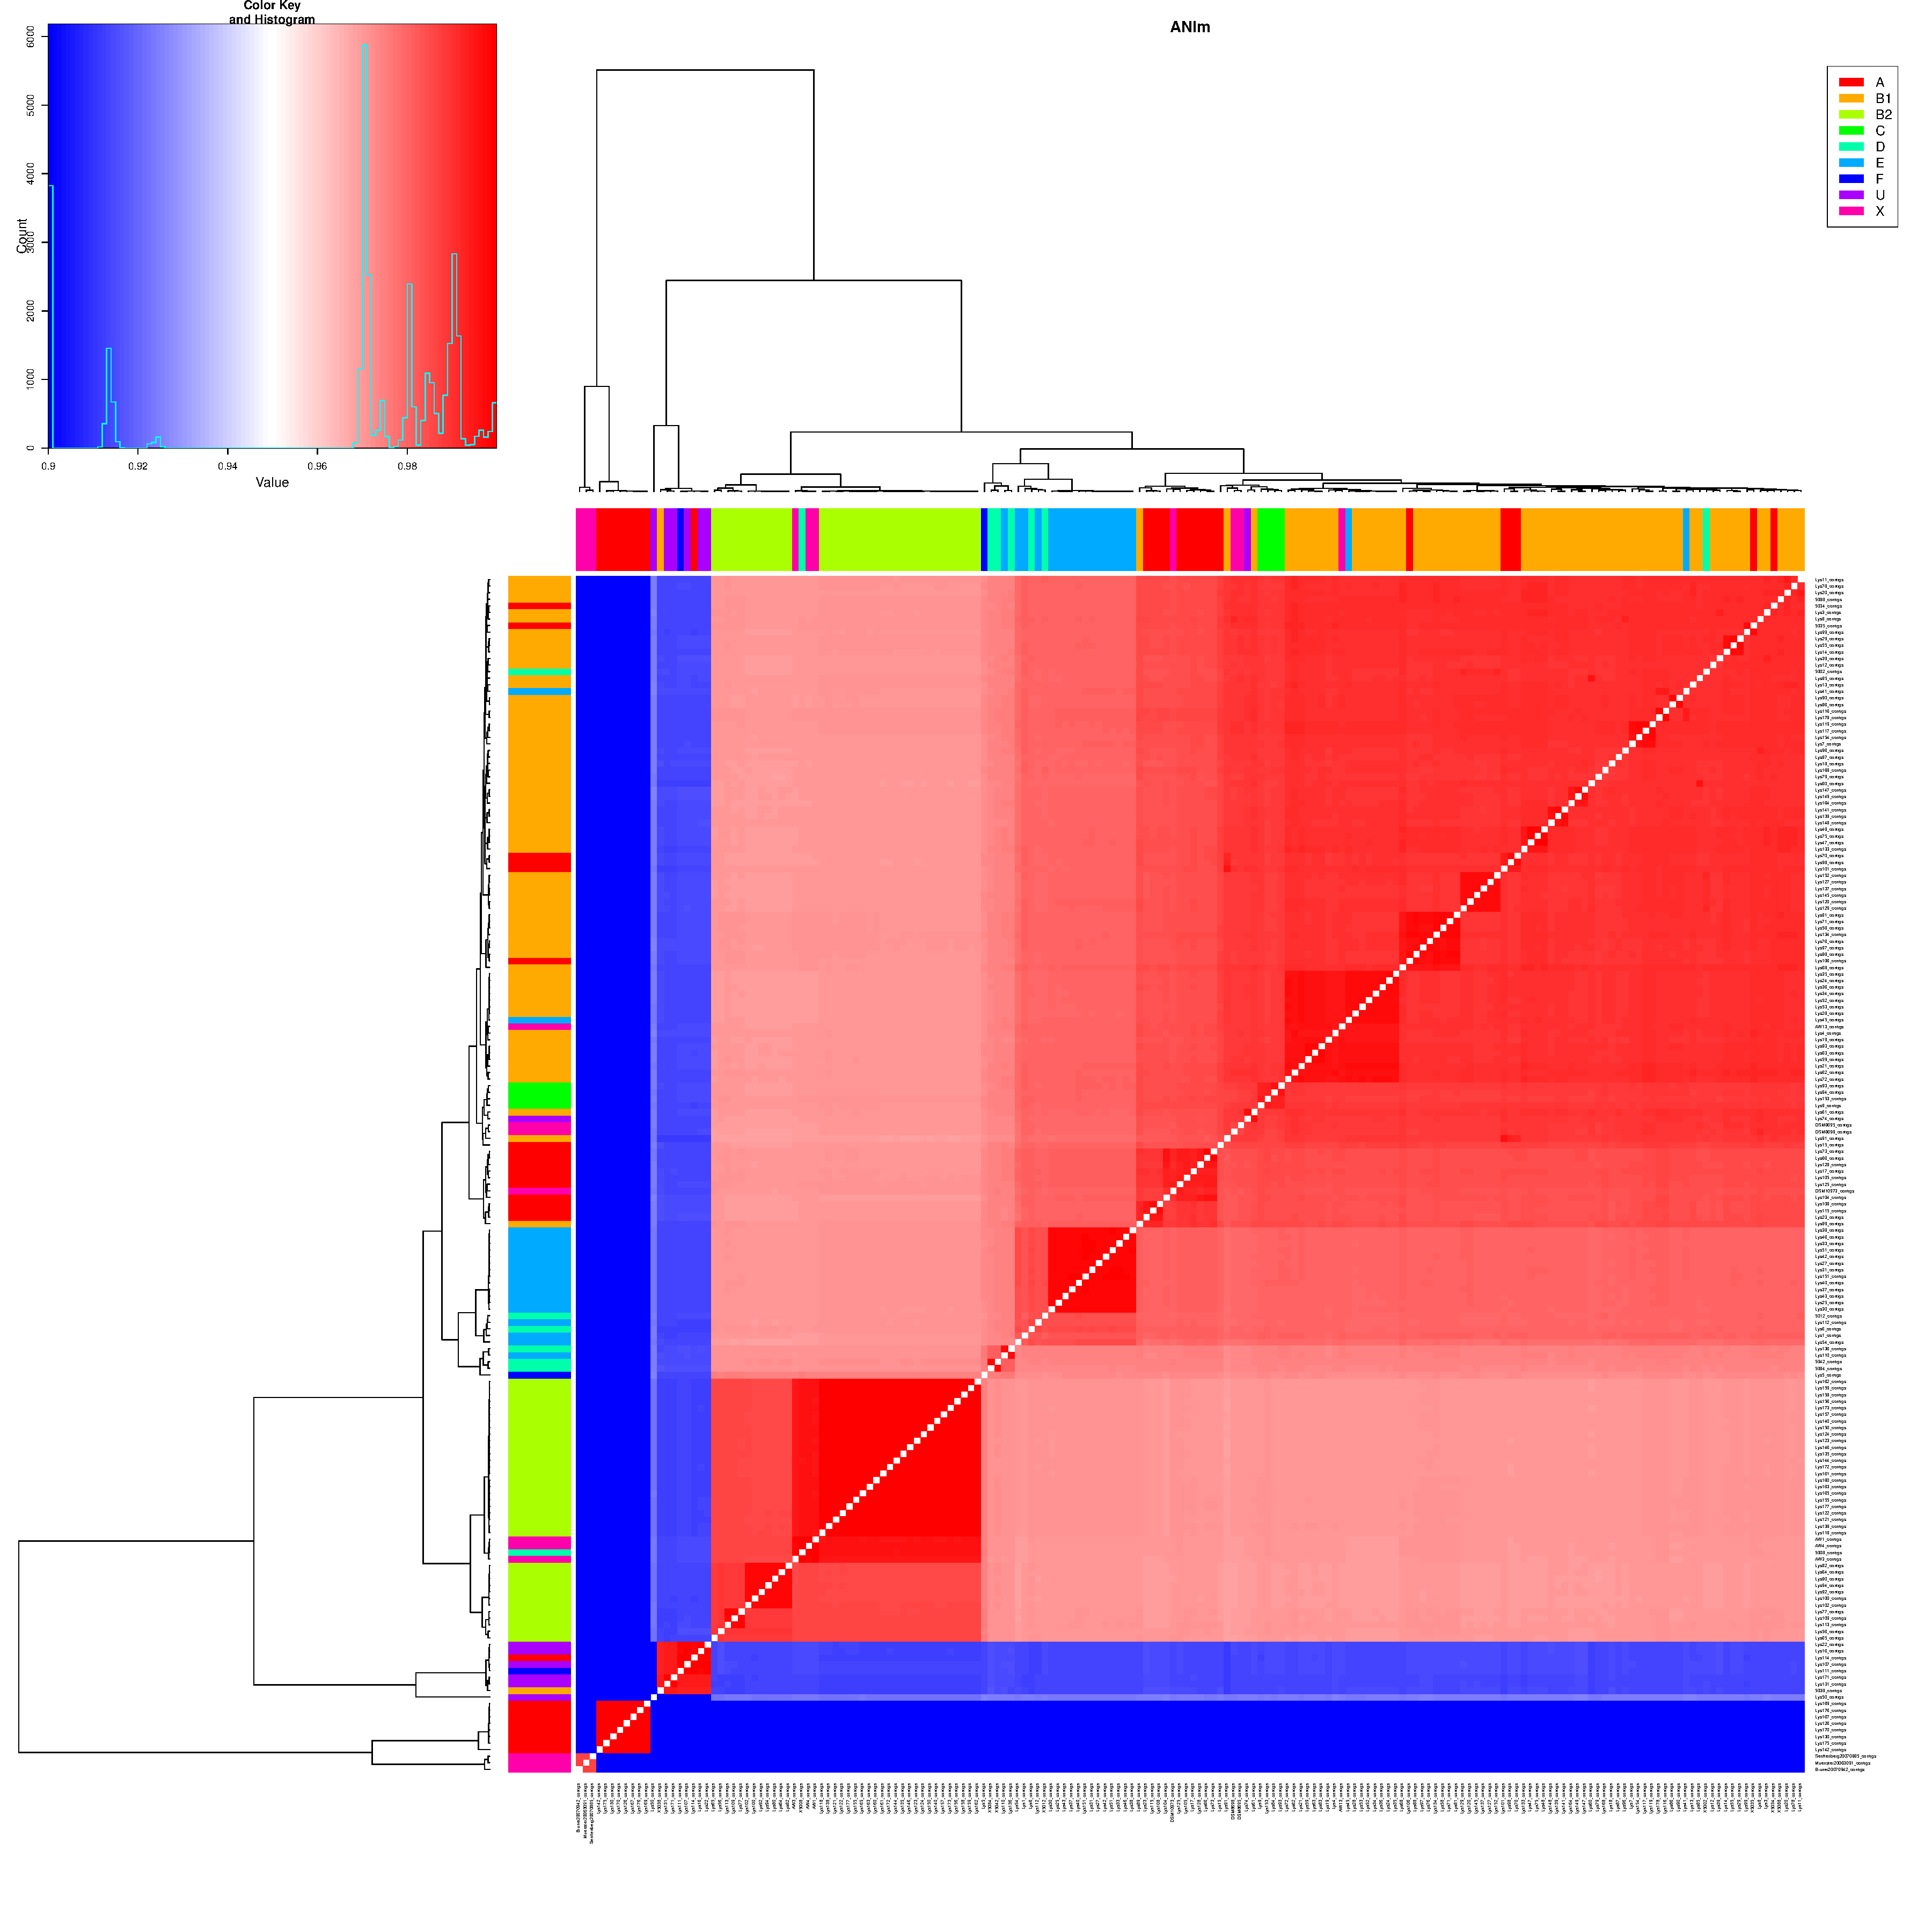
\includegraphics[width=0.65\textwidth]{images/ANIm_Ecoli}
  \end{center}      
\end{frame}

% Campy sequencing summary
\begin{frame}
  \frametitle{2014: \textit{Campylobacter} spp.}
  Sequenced $\approx$ 1034 isolates of \textit{Campylobacter} \\
  Clinical, animal, food-associated isolates
  \begin{itemize}
    \item Illumina paired-end sequencing. \textbf{Total cost of sequencing $>$1000 bacteria: $\approx$\pounds60k}
    \item \textbf{Automated annotation: PRODIGAL}    
  \end{itemize}      
  \begin{center}
    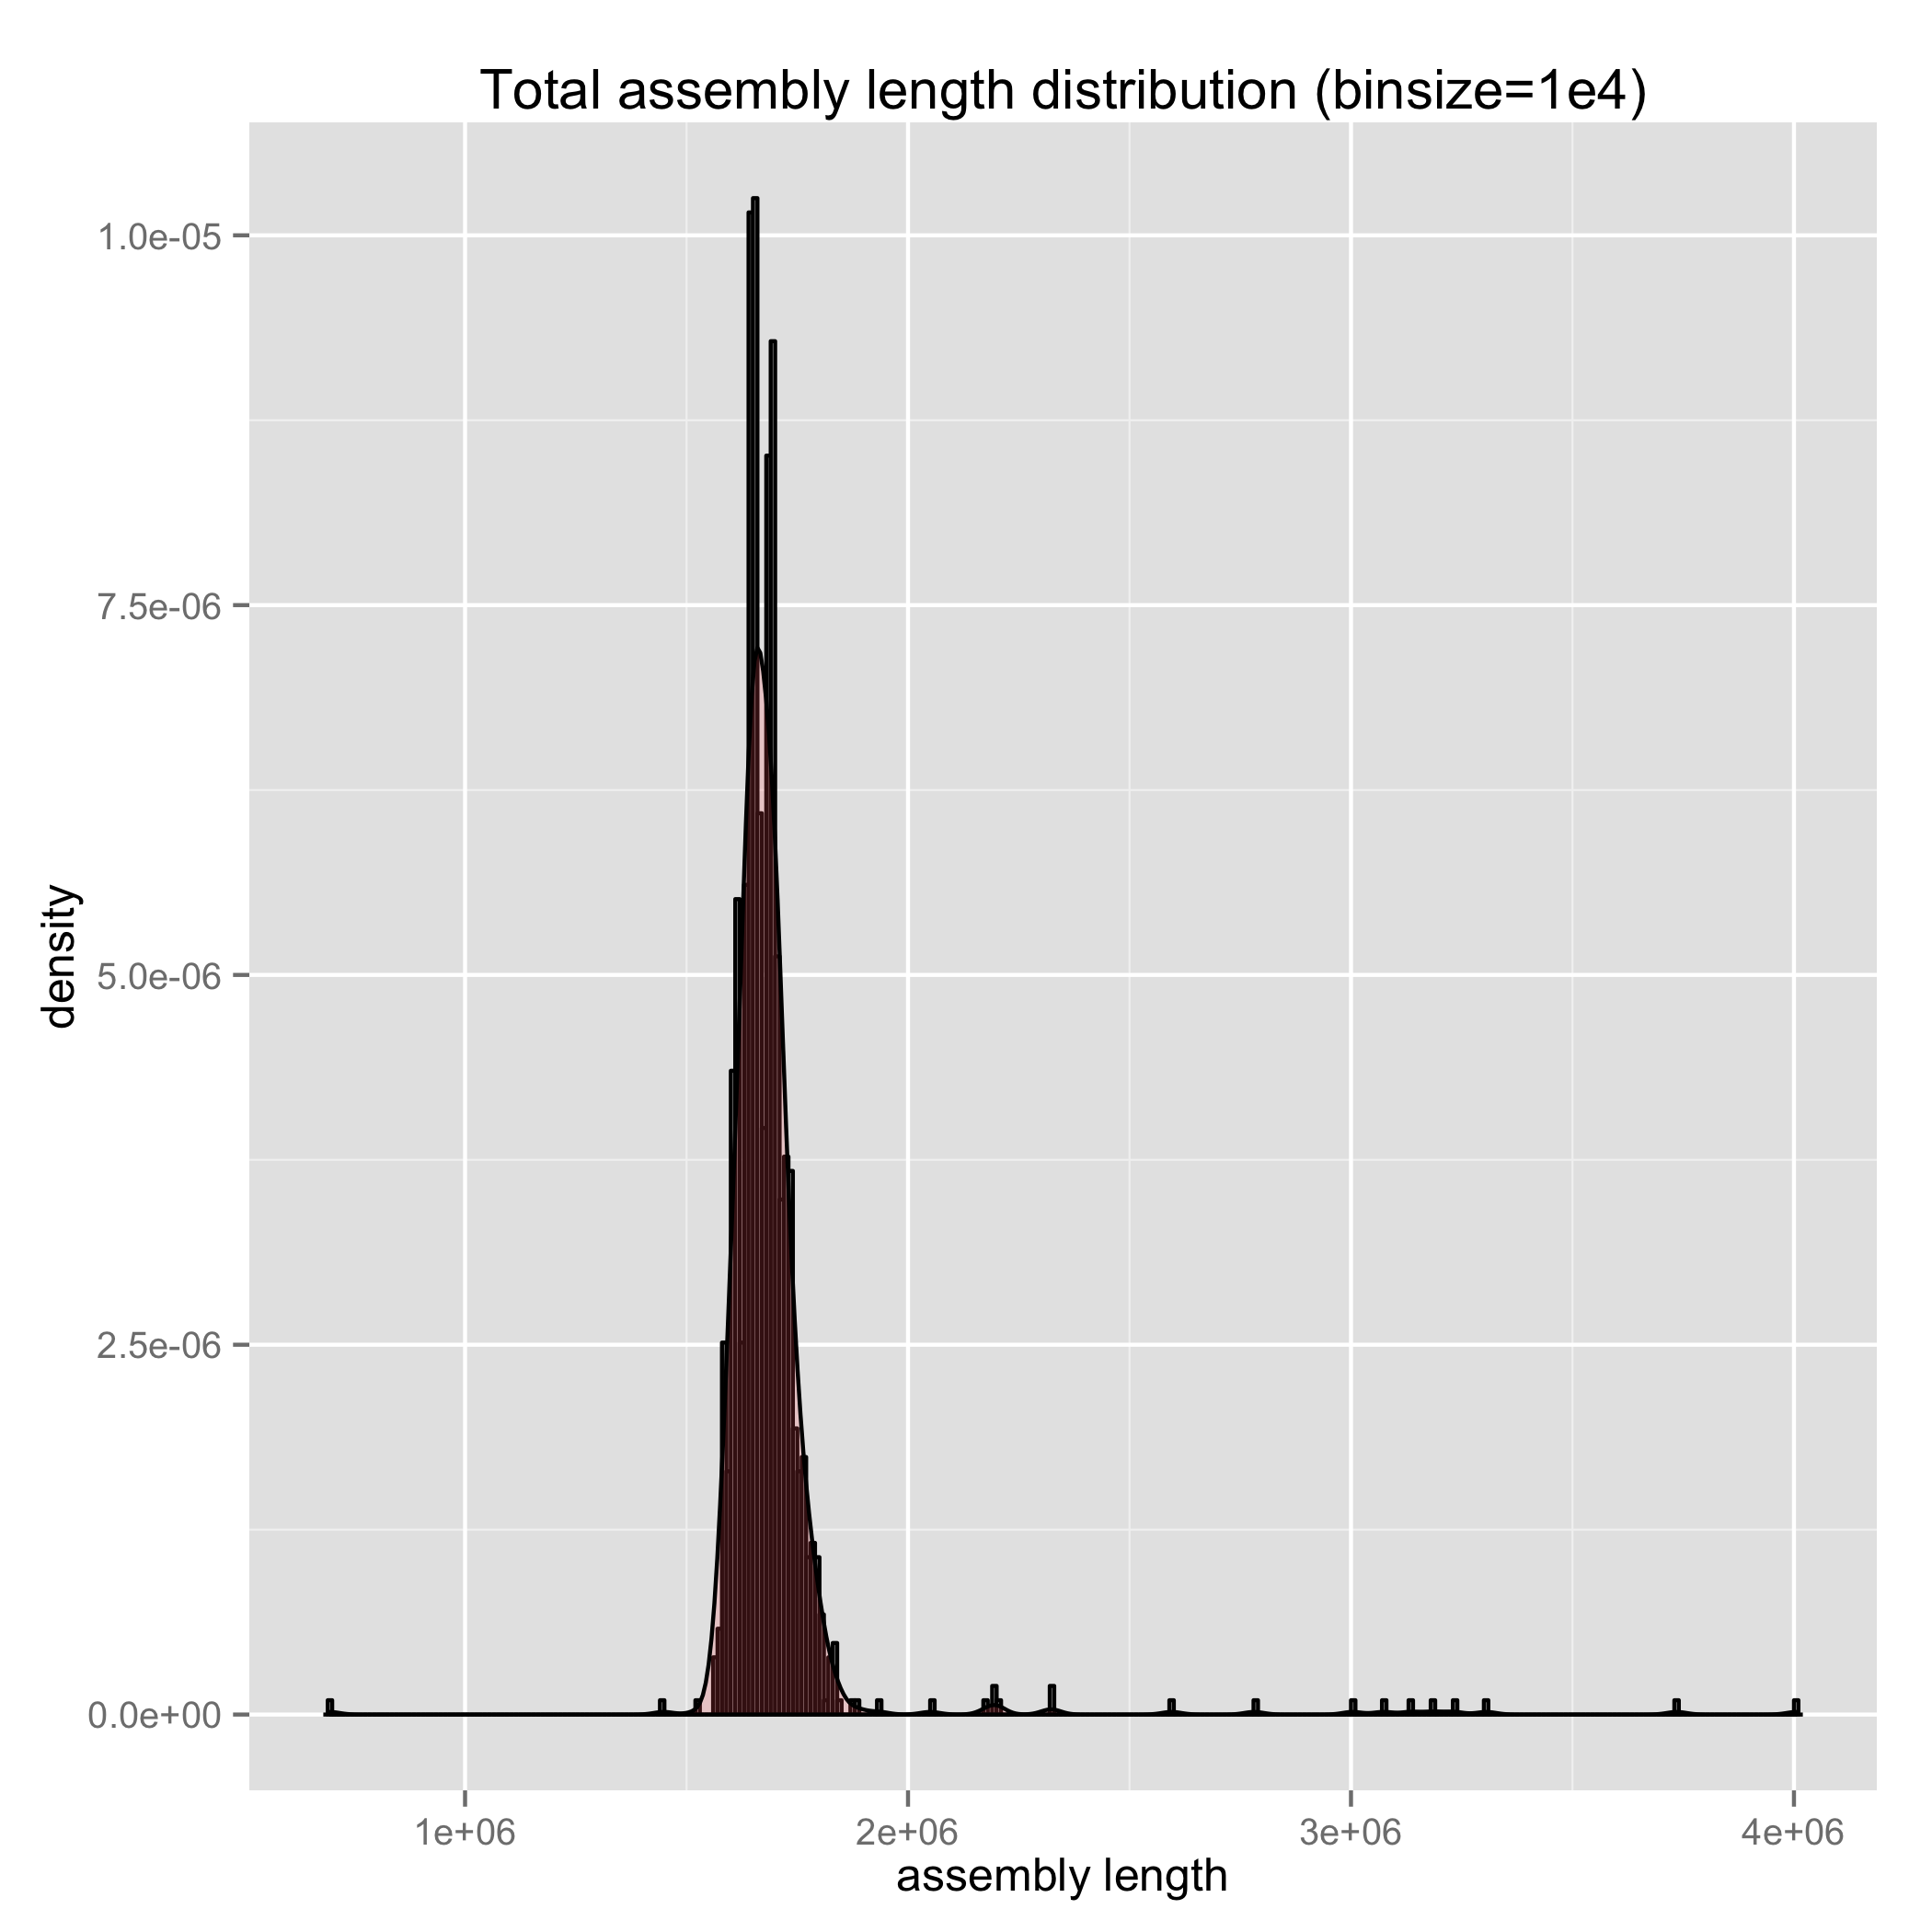
\includegraphics[width=0.4\textwidth]{images/Asm_long_contigs_length_histogram}
  \end{center}        
\end{frame}

% Campy genecalling summary
\begin{frame}
  \frametitle{2014: \textit{Campylobacter} spp.}
  \begin{itemize}
    \item Identified 15554 gene families from genecalls.
    \item To calculate, took 23 days on institute cluster (4e12 pairwise protein comparisons!).  
  \end{itemize}      
  \begin{center}
    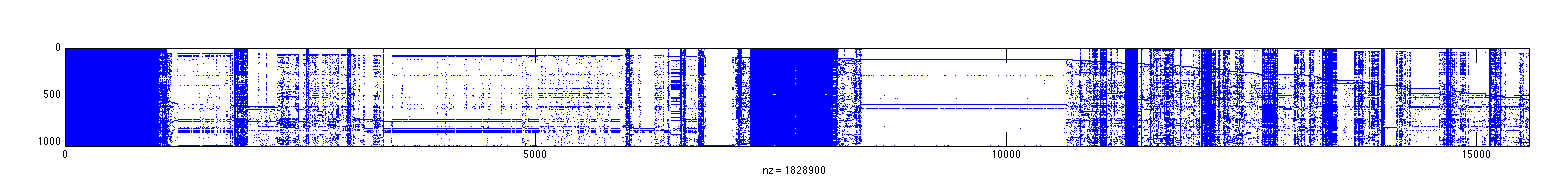
\includegraphics[width=1\textwidth]{images/Pres_abs_mat} \\
    
\includegraphics[width=0.4\textwidth]{images/campy_presence_absence}    
  \end{center}        
\end{frame}

% SUBSECTION: What's changed?
% What are the major changes that 
\subsection{So what's changed?}

% High-throughput sequencing totally changed everything
\begin{frame}
  \frametitle{So what's changed?}
  \begin{itemize}
    \item \textbf{Cost}: \pounds250k per genome, to \pounds60 per genome. \\
             \textbf{Now cheaper to sequence a genome than to analyse it!}
    \item \textbf{Location}: sequencing centre, to benchtop
    \item \textbf{Data}: volume has increased massively - what you get back from machines, and what's out there to work with\\
             \textbf{More data is better, but also more challenging.}
    \item \textbf{Speed}: typical sequencing run time can be less than a day
    \item \textbf{Software}: more software to do more things (but not always better$\ldots$)
    \item New kinds of \textbf{experiment}: genomes, exomes, variant calling, methylated sequences, $\ldots$
    \item New kinds of \textbf{application}: diagnostics, epidemic tracking, metagenomics, $\ldots$
  \end{itemize}       
\end{frame}

% More power for comparative genomics
\begin{frame}
  \frametitle{So what's changed?}
  Having a single genome is useful, but having thousands really helps \textbf{\textit{comparative genomics}}: \\
  combining genomic data, evolutionary and comparative biology
  \begin{itemize}
    \item Transfer functional understanding of model systems (e.g. \textit{E. coli}) to non-model organisms
    \item Genomic differences may underpin phenotypic (host range, virulence, physiological) differences
    \item Genome comparisons aid identification of functional elements on the genome
    \item Studying genomics changes reveals evolutionary processes and constraints
  \end{itemize}       
\end{frame}

